\chapter{Statistical Analysis}\label{sec:statistics}
Scientific investigations generally start with a hypothesis, which is then tested against empirical data. This chapter focuses on the frequentist statistical methods used to evaluate whether the observed collision data support or contradict the proposed hypothesis.

Central to this discussion is the concept of the p-value, which arises within hypothesis testing. The p-value quantifies the compatibility of the observation with the assumption and is particularly important in \ac{hep}, to confidently determine if a hypothesized process is realized in nature.

Specifically for this task in \ac{hep}, the \textsc{histfactory} framework has been developed. This section the fundamentals of the approach and its implementation \citep{pyhf,pyhf_joss}. The following is based on \citep{cowan2011asymptotic,behnke2013data,pyhf}.



\section{Profile Likelihood Ratio}\label{sec:likelihood}
The statistical model needs to reflect the compatibility of predictions with the observed collision events. This can be quantified by a likelihood function $L(\bm{x} | \bm{\phi})$ which can be understood as a probability measure for an observation $\bm{x}$ under a given set of parameters $\bm{\phi}$. In this counting experiment, histograms are the primary tool of analysis.

% The observation $\bm{x}=(\bm{n},\bm{a})$ can be subdivided into observable histograms $\bm{n}$ and $\bm{a}$ auxiliary measurement histograms that assist in constraining the model and usually amount to considered uncertainties. Another useful splitting for the set of parameters is $\bm{\phi}=(\bm{\psi},\bm{\Theta})$ into so-called parameters of interest $\bm{\psi}$ and nuisance parameters $\bm{\Theta}$. For this section only one parameter of interest is considered, the signal strength $\mu$.

The set of parameters $\bm{\phi}$ is divided into a parameter of interest $\mu$, usually corresponds to the signal strength and nuisance parameters $\bm{\Theta}$ that add degrees of freedom to the model. For a single signal and background contribution counted with a histogram in some observable the expected counts per bin can be expressed in terms of the expected signal $s_i(\bm{\Theta})$ and background $b_i(\bm{\Theta})$ in bin $i$, both dependent on the nuisance parameters. The expected count per bin of the observable $n_i$ can then be expressed as
\begin{equation} \label{eq:n_i}
    \langle n_i\rangle = \mu s_i(\bm{\Theta}) +b_i(\bm{\Theta}).
\end{equation}
% Similarly for auxiliary measurement bin.s $a_i$ their expectation value are calculable from some function $u_i(\bm{\Theta})$ modeling some observable and is also dependent on the nuisance parameters
% \begin{equation} \label{eq:a_i}
%     \langle a_i(\bm{\Theta}) \rangle = u_i(\bm{\Theta}).
% \end{equation}
Given that events occur at a constant rate and independently in time, each bin follows a Poisson distribution:
\begin{equation}\label{eq:poisson}
    P(r,k)=\frac{r^k e^{-r}}{k!},
\end{equation}
where $r$ is the expected rate of occurrences (the prediction) and $k$ is the observed occurrences. A likelihood can then be constructed from a product of the Poisson probabilities and additional terms $c_k$ that help in constraining the model
\begin{equation}\label{eq:likelihood}
    L(\mu,\bm{\Theta})=
    \prod_{j=1}^N \frac{(\mu s_j(\bm{\Theta}) + b_j(\bm{\Theta}))^{n_j}}{n_j !} e^{-(\mu s_j(\bm{\Theta}) + b_j(\bm{\Theta}))}
    \prod_{k=1}^M c_k(\bm{\Theta}).
\end{equation}
These constraint terms can be interpreted as penalties on the likelihood, incorporating prior knowledge into the model. For instance, they can represent another Poisson measurement where only the background is expected, or be used to account for uncertainties, as discussed in detail in Section \ref{sec:histfactory_model}.

To test a hypothesized value of $\mu$, the best choice according to the Neyman-Pearson lemma, is the profile likelihood ratio. This ratio reduces the dependence of the likelihood function to the parameter of interest:
\begin{equation}\label{eq:likelihood_ratio}
    \lambda(\mu)=
    \frac{L(\mu,\hat{\hat{\bm{\Theta}}})}
    {L(\hat{\mu},\hat{\bm{\Theta}})}.
\end{equation}
Here, the denominator is the unconditional maximum likelihood estimate, allowing both $\hat{\mu}$ and $\hat{\bm{\Theta}}$ to vary freely to maximize $L$. The numerator is the maximum likelihood conditioned on some chosen $\mu$ and the set of nuisance parameters $\hat{\hat{\bm{\Theta}}}$ that maximize the likelihood for that particular $\mu$. This definition gives $0 \leq \lambda \leq 1$ where $\lambda = 1$ corresponds to perfect agreement of the hypothesized value of $\mu$ with the model.

\section{Test Statistic and p-value}

To test for a given hypothesis a test statistic serves a quantity that reduces the data set to one value on which the hypothesis is conducted. The test statistic here is a transform of the profile likelihood
\begin{equation}
    t(\mu)=-2\ln \lambda(\mu).
\end{equation}
This translates to $t \rightarrow 0$ as increasing agreement and $t \rightarrow \infty$ as decreasing agreement to the model. A right-tail p-value can then be calculated from the probability density of the test statistic $f(t | \mu)$ as
\begin{equation}\label{eq:p-value}
    p= \int_{t_\text{obs}}^{\infty}
    f(t | \mu) \mathrm{d}t
\end{equation}
Here, $t_\text{obs}$ is the test statistic $t$ computed using the particular $\mu$ and observed data. The probability density function $f(t | \mu)$ of the test statistic $t$ quantifies how probable a particular value of $t$ is under a fixed value of the signal strength $\mu$, essentially measuring how frequently a particular value of $t$ occurs in comparison to all other possible values.

The specific form of the test statistic is useful due to existing approximations for $f(t | \mu')$ with $\mu'$ as the true strength parameter \citep{cowan2011asymptotic}. \citet{wald1943tests} demonstrated that for a single parameter of interest, the test statistic asymptotically approaches  a squared distance between the tested parameter $\mu$ and its maximum likelihood estimate $\hat{\mu}$
\begin{equation}
    t(\mu)=-2\ln \lambda(\mu)=
    \left(\frac{\mu-\hat{\mu}}{\sigma_{\hat{\mu}}} \right)^2
    + \mathcal{O}(\frac{1}{\sqrt{N}}),
\end{equation}
where $\hat{\mu}$ is normally distributed around its true value $\mu'$ with standard deviation $\sigma_{\hat{\mu}}$. $\hat{\mu}$ is determined by the maximum likelihood fit and the standard deviation is taken from the covariance matrix of the maximum likelihood estimates of the nuisance parameters $V_{ij}(\hat{\bm{\Theta}})$, detailed in \ref{sec:unc_extraction}.

With this result, it can be shown that if $\hat{\mu}$ is Gaussian distributed, the probability density function of $t$ follows a \textit{non-central $\chi^2$ distribution} in the large sample limit
\begin{equation}\label{eq:chi-square}
    f(t | \mu)=\frac{1}{2\sqrt{t}}\frac{1}{\sqrt{2\pi}}
    \left[
        \exp\left(-\frac{1}{2}\left(\sqrt{t}+\sqrt{\Lambda}_\mu\right)\right)
        +
        \exp\left(-\frac{1}{2}\left(\sqrt{t}-\sqrt{\Lambda}_\mu\right)\right)
        \right],
\end{equation}
with non-centrality parameter
\begin{equation}
    \Lambda_\mu=\frac{(\mu-\mu')^2}{\sigma^2}.
\end{equation}
Figure \ref{fig:test_stat_example} illustrates these steps. $\Lambda_\mu$ is estimated by setting the observed values to the predicted ones, such that the true value $\mu'$ in $\Lambda_\mu$ becomes the maximum likelihood estimate one $\hat{\mu}$. which results. The dataset that achieves this, with observed event counts per bin exactly matching the predicted ones, is referred to as the 'Asimov' dataset.

\begin{figure}
    \centering
    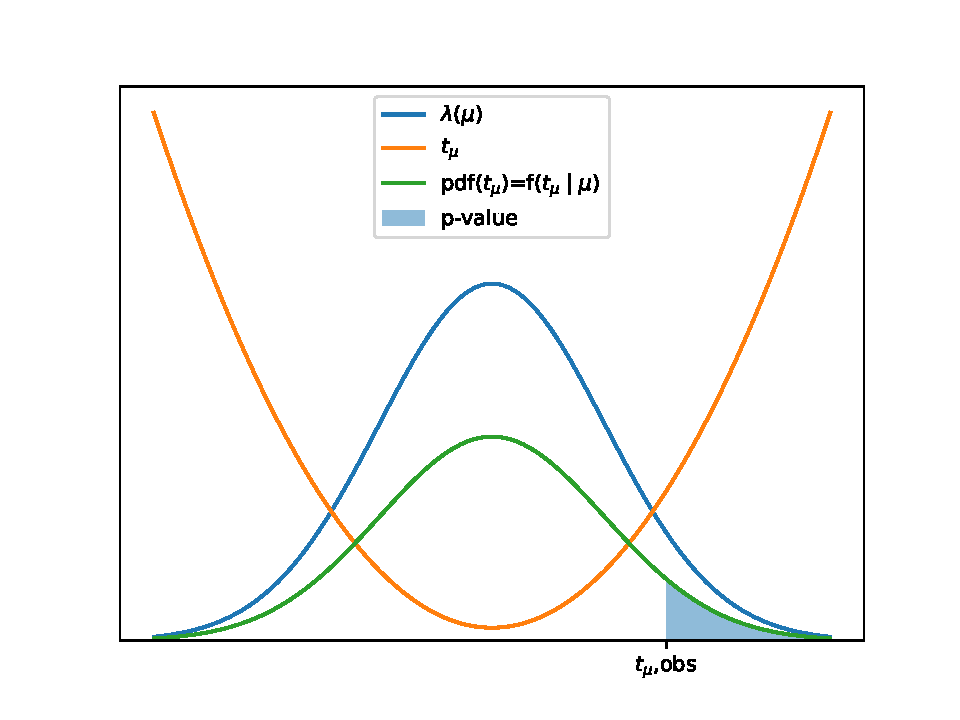
\includegraphics[width=0.8\textwidth]{test_stat_example.pdf}
    \caption[]{A sketch to follow the steps to calculate p-values. (\textbf{left}) The profile likelihood ({\color[HTML]{1f77b4}{$\bm{\diagup}$}}) has essentially some hill-like form with a maximum at ${\lambda(\hat{\mu},\hat{\bm{\Theta}})}$. The test statistic $t$ ({\color[HTML]{ff7f0e}{$\bm{\diagup}$}}) is calculated as $-2\mathrm{ln}(\lambda)$. (\textbf{right}) For one parameter of interest in the large sample limit $f(t | \mu)$ from equation \ref{eq:chi-square} follows a non-central chi-squared distribution with one degree of freedom. The blue shaded area under the probability density functions is a right hand sided p-value.}
    \label{fig:test_stat_example}
\end{figure}

The ability to compute p-values allows scientists to state the likelihood that the proposed hypothesis is supported by the observed data. Specifically, the p-value indicates the probability of obtaining data at least as extreme as the observed data if the experiment were repeated many times. This measure reflects the degree of incompatibility between prediction and observation.

In the scientific community, a p-value of 0.05 is commonly accepted as significant. However, particle physicists usually transform the p-value into a significance using the inverse cumulative distribution function of the standard normal distribution:
\begin{equation}
    Z = \Phi^{-1}(1 - p).
\end{equation}
Thus, the p-value is expressed in terms of the number of standard deviations if the test statistic were normally distributed.
The found p-value is thus expressed in terms of the number of standard deviations this p-value would have if the test statistic were standard normal distributed. Particle physicists claim discovery of a new phenomenon for $Z>5$ ($p$ < \qty{2.87e-7}{}) and exclude hypotheses for $Z>2$ ($p$ < 0.05). The Asimov significance, an estimate for the significance, can be calculated from the counts per bin when setting observed data points to the expected number of events predicted by the model:
\begin{equation}\label{eq:asimov-significance}
    Z_A = \sqrt{2\sum_{i\in bins}((s_i + b_i)(\log{(1 + s_i / b_i)}) - s_i)}.
\end{equation}


A key consideration is that $t$ can assume negative values for $\mu$ which might be non-physical depending on the context. This is managed by cutting off the test statistic for undesired behavior. For instance, an adjusted test statistic for setting upper limits is:
\begin{equation}
    q_\mu=
    \begin{cases}
        -2\ln \lambda(\mu) & \hat{\mu}\leq\mu \\
        0                  & \hat{\mu}> \mu
    \end{cases}.
\end{equation}
Here, if a tested signal strength $\mu$ is not larger than the maximum estimate, it is not regarded as less compatible and is set to zero. Various cases and approximations of probability density functions in different scenarios are detailed in \citep{cowan2011asymptotic}.

\section{The CL$_s$ Value}\label{sec:cls}
Particle physicists typically concentrate on two key aspects when performing statistical tests to discover new phenomena: the accurate modeling of known backgrounds and whether there is evidence in the observations for a new phenomenon. This involves assessing two distinct hypotheses: a background only ($b$) and one that involves signal and background ($s+b$). Each will result in a p-value of their own.

To combine these two aspects into a unified metric particle physicists developed the CL$_s$ quantity. This measure not only considers the potential presence of new phenomena but also the accuracy of the background modeling.
\begin{equation}
    \mathrm{CL}_s=\frac{p_{s+b}}{1-p_{b}}=
    \frac
    {\int_{t_\text{obs}}^{\infty}
        f(t_{s+b} | \mu) \mathrm{d}t}
    {1-\int_{t_\text{obs}}^{\infty}
        f(t_{b} | \mu) \mathrm{d}t}.
\end{equation}
The numerator represents the p-value for the alternative hypothesis while the denominator penalizes the $p_{s+b}$ based on the compatibility of the background model with observed data. For example, $p_{b} = 0$ indicates a perfect modeling of backgrounds. This becomes particularly useful in searches with poor sensitivity as the hypothesis test depends crucially on the background estimate. When for instance the background is underestimated, the background only $p_b$-value would be large and would penalize $p_{s+b}$. The concept can also be understood visually from the first figure of the paper that introduced the CL$_s$ quantity \citep{read2002presentation} as explained
in figure \ref{fig:cls}.
\begin{figure}
    \centering
    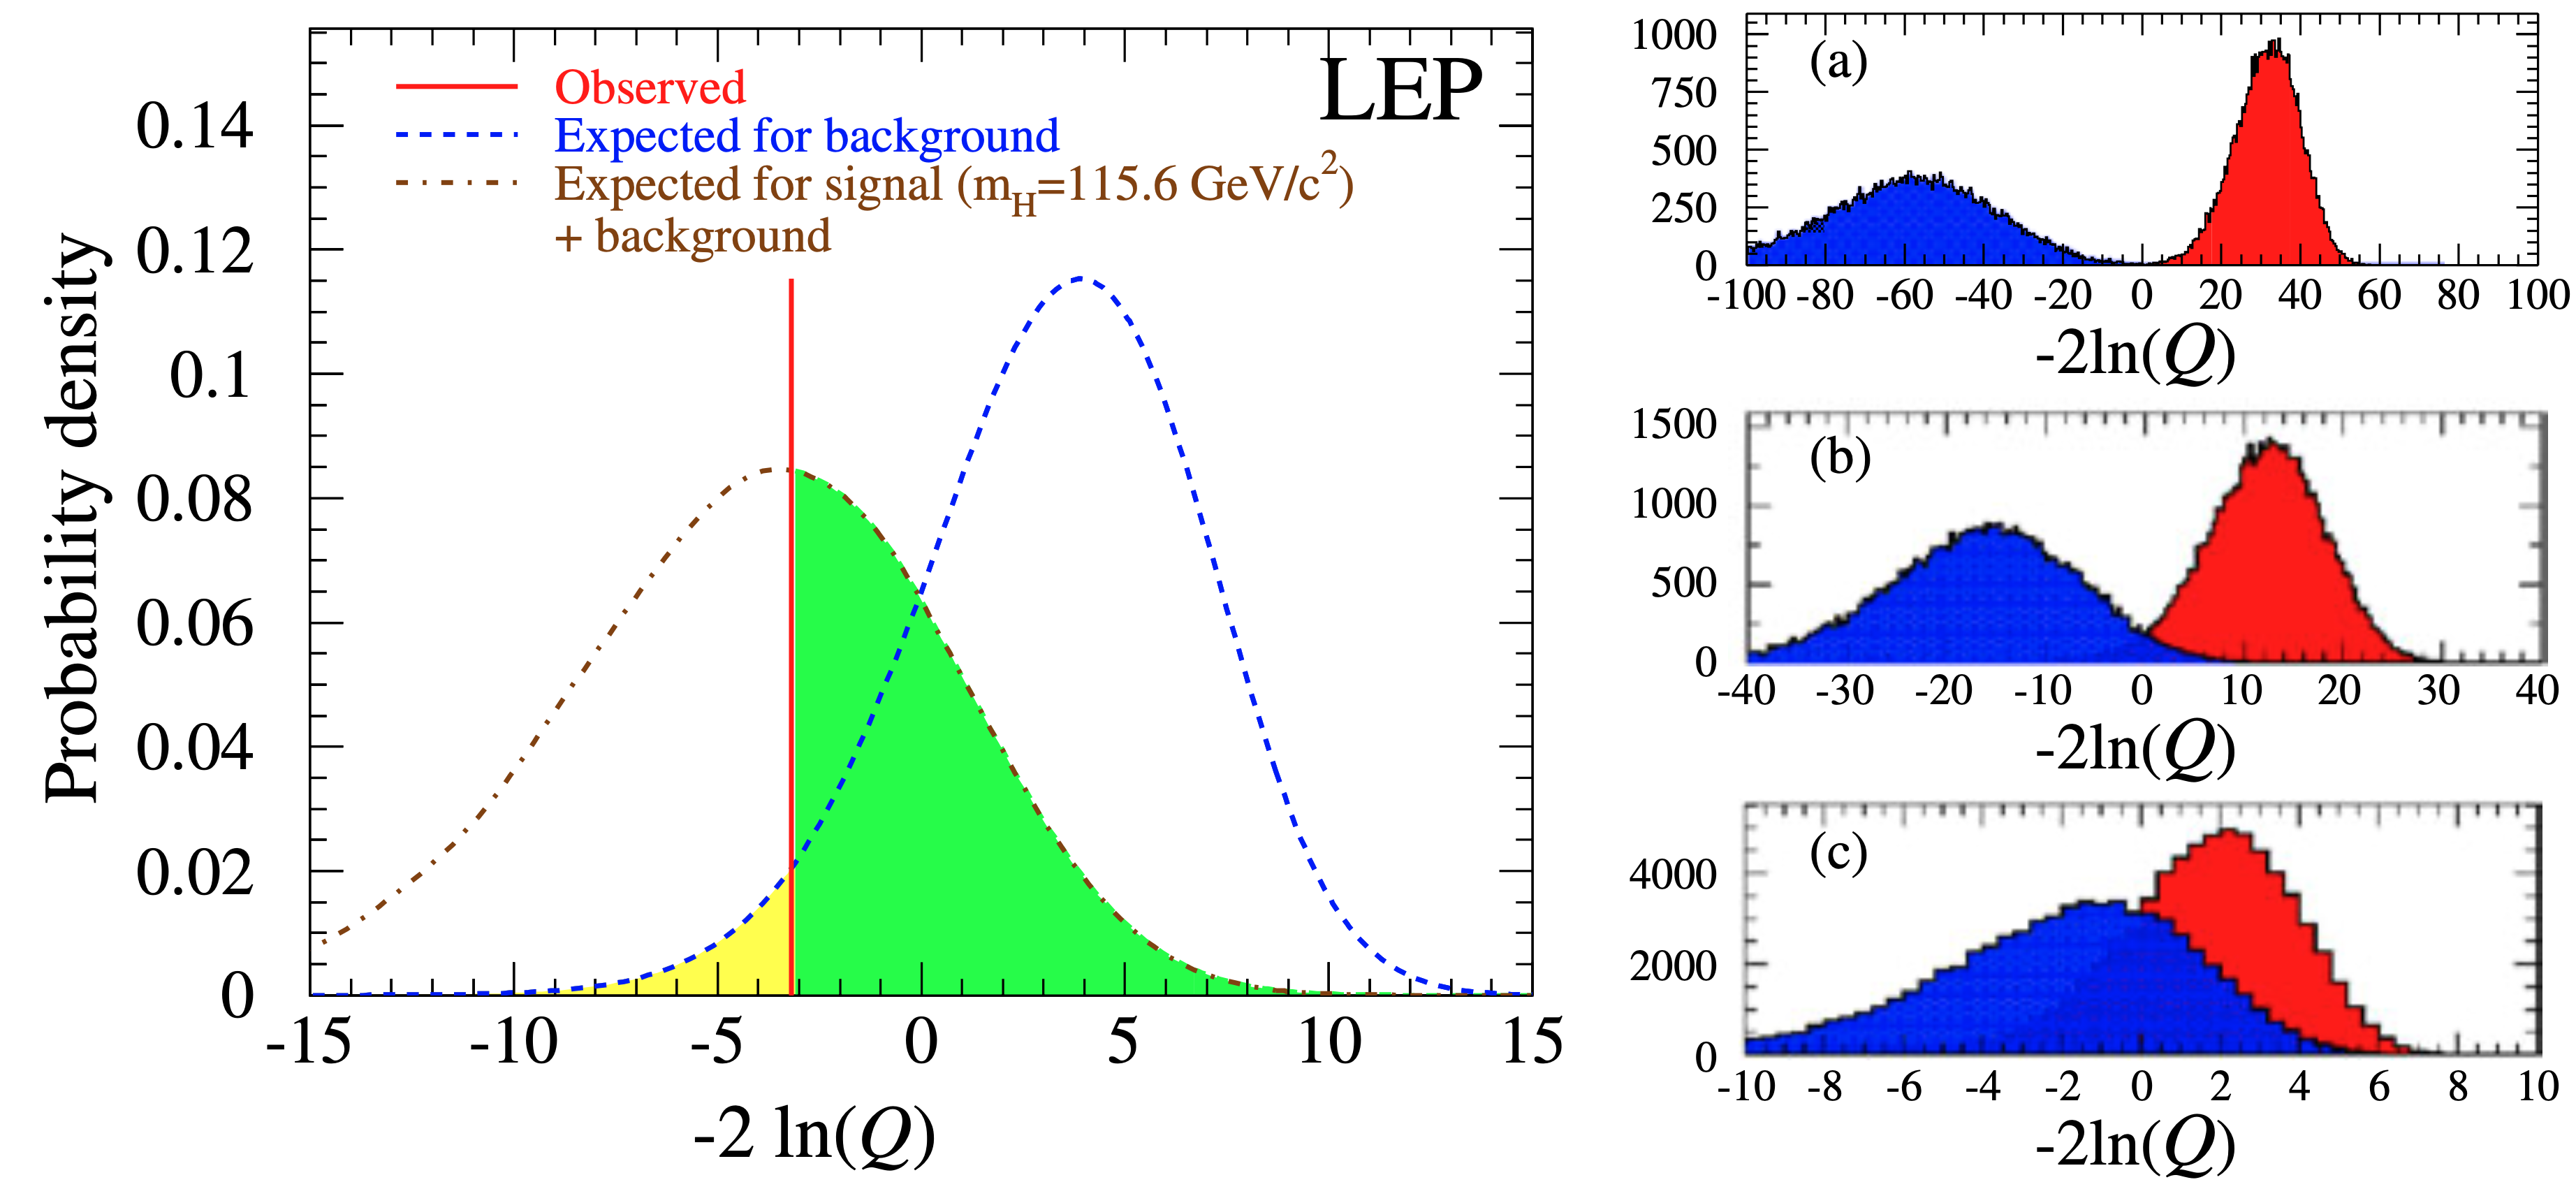
\includegraphics[width=1\textwidth]{cls.png}
    \caption[]{Probability density functions of test statistics from a Higgs search at LEP, illustrating p-value calculations ($\lambda$ from the full text becomes $Q$). (\textbf{left}) The probability density functions of the test statistic $f(t | \mu)$ of the signal + background ({\color[HTML]{804000}{$\bm{\diagup}$}}) and background only ({\color[HTML]{2100FF}{$\bm{\diagup}$}}) hypotheses. The p-value is calculated by integration from $t_\text{obs}$ (the red observed line ({\color[HTML]{FF0000}{$\bm{\diagup}$}})) to infinity (see eq. \ref{eq:p-value}). The green shaded area (\hexbox{00FF00}) corresponds to $p_{s+b}$ whereas the yellow area (\hexbox{FDFF02}) corresponds to $1-p_b$ since $\int \mathrm{pdf}=1$. (\textbf{right}) Degradation of search sensitivity from (a) to (c). Note the color change in probability density functions: signal + background (\hexbox{2100FF}) and background only (\hexbox{FF0000}).For example given an observation of ($t_\text{obs}\approx0$), yields for plot (a) $p_{b}\approx 1$ and $p_{s+b}\approx 0$ resulting in a CL$_s\approx 0$; with increasing overlap the CL$_s$ value increases and the sensitivity decreases. Adopted from \citep{read2002presentation}.}
    \label{fig:cls}
\end{figure}


\section{HistFactory}\label{sec:histfactory_model}
A widely-used model in \ac{atlas} for constructing likelihoods, as discussed in section \ref{sec:likelihood} is known as HistFactory \citep{cranmer2012histfactory}. It simplifies building a likelihood by breaking it down into fundamental components and considering different categories of model parameters $\bm{\phi}$.

\newcommand{\freeset}{\bm{\eta}}
\newcommand{\constrset}{\bm{\chi}}
\newcommand{\singleconstr}{\chi}
\newcommand{\channelcounts}{\bm{n}}
\newcommand{\auxdata}{\bm{a}}
\newcommand{\poiset}{\bm{\psi}}
\newcommand{\nuisset}{\bm{\theta}}
\newcommand{\fullset}{\bm{\phi}}
\newcommand{\singlefull}{\phi}
\begin{equation}
    L(\bm{x}|\fullset) \quad=\quad
    L(\bm{x}|\overbrace{\poiset}^{\llap{\text{parameters of interest}}},\underbrace{\nuisset}_{\llap{\text{nuisance parameters}}}) \quad=\quad
    L(\bm{x}|\overbrace{\freeset}^{\rlap{\text{free}}},\underbrace{\constrset}_{\rlap{\text{constrained}}}),
\end{equation}
HistFactory distinguishes between free parameters $\freeset$ and constrained parameters $\constrset$, which are used to implement uncertainties into the likelihood. There may be several histograms of an observable, measured in orthogonal kinematic regions, called channels $c$, with bins indexed by $b$. Constraint terms are denoted by $c_{\singleconstr}$. The likelihood is described as:
\begin{equation}
    L(\channelcounts, \auxdata \,|\,\freeset,\constrset)
    = \underbrace{{\prod_{c\in\mathrm{\,channels}} \prod_{b \in \mathrm{\,bins}_c}
                \textrm{Pois} (
                \;\overbrace{n_{cb}}^{\llap{\text{\strut observed}\quad\;}}
                \,|\, \overbrace{\nu_{cb}\left(\freeset,\constrset\right)}^{\llap{\quad\text{\strut predicted}}}
                \;)}}_{\substack{\text{Simultaneous measurement}\\%
            \text{of multiple channels}}}
    \underbrace{{\prod_{\singleconstr \in \constrset} c_{\singleconstr}(a_{\singleconstr} |\, \singleconstr)}}_{\substack{\text{constraint terms}\\%
            \text{for }\text{auxiliary measurements}}}.
    \label{eq:histfactory_likelihood}
\end{equation}

Here, $\bm{n}$ represents observed and $\bm{a}$ auxiliary measurement histograms. The $n_{cb}$ enter the Poisson term per bin and channel, and the predicted counts per bin are governed by the free and constrained parameters $\nu_{cb}(\freeset,\constrset)$. Functions $c_{\singleconstr}(a_{\singleconstr} |, \singleconstr)$ penalize the likelihood $L$ with uncertainties $a_\chi$ to constrain the parameter $\singleconstr$, as discussed in detail in section \ref{sec:modifiers}.

\subsection{Modifiers}\label{sec:modifiers}
The prediction is a sum of nominal counts per bin $\nu_{scb}^0$ over all samples $s$ (e.g., $t\overline{t}$, multijet-background, etc.). These nominal counts per bin are subject to uncertainties and have some degree of freedom. This modification to the likelihood is taken into account via the constraint terms, which penalize the likelihood proportional to the modification. There are multiplicative $\kappa_{scb}$ and additive modifiers $\Delta_{scb}$ to the nominal bin count $\nu_{scb}^0$:

\begin{align}
    \nu_{cb}\left(\freeset,\constrset\right) & = \sum_{s\in\mathrm{\,samples}} \nu_{scb}\left(\freeset,\constrset\right)                                                                                                \\
                                             & = \sum_{s\in\mathrm{\,samples}} \underbrace{\left(\prod_{\kappa\in\,\bm{\kappa}} \kappa_{scb}\left(\freeset,\constrset\right)\right)}_{\text{multiplicative modifiers}} \nu_{scb}^0 +
    \underbrace{\sum_{\Delta\in\bm{\Delta}} \Delta_{scb}\left(\freeset,\constrset\right)}_{\text{additive modifiers}}.
    \label{eq:modifier_equation}
\end{align}    
Considering one nuisance parameter $\chi$ controlling a multiplicative modifier $\kappa_{scb}(\chi)$ on $\nu_{scb}^0$, an optimum can be found by modifying the prediction to move closer to the observed value while keeping the constraint term controlled by the same $\chi$ at values where the penalization of the likelihood remains insignificant.

Histfactory implements various types of modifiers detailed in \citep{pyhf_intro,heinrich2019searches,cranmer2012histfactory}. The ones used in this work include a free rate modifier for the signal strength $\mu$ that affects all bins equally:
\begin{equation}
    \nu_{scb}(\mu)=\mu \nu_{scb}^0,
\end{equation}
and inter-/extrapolation functions $I(\alpha)$ depending on a nuisance parameter $\alpha$ that continuously scale the nominal counts per bin for a given uncertainty. The modifiers control the nominal bin count $\nu_{scb}$ such that $\alpha=\pm 1$ results in to 1 standard deviation uncertainties:
\begin{equation}
I(\alpha=\pm 1) \nu_{scb}^0=\nu_{scb}^\pm.
\end{equation}
These modifications are accompanied by a Gaussian constraint term to the likelihood:
\begin{equation}
    \text{Gaus}(\mu|x,\sigma)=\frac{1}{\sigma\sqrt{2\pi}}e^{-\frac{1}{2}\left(\frac{x-\mu}{\sigma}\right)^2}.
\end{equation}
This constraint term is scaled to one standard deviation $\sigma$ controlled by the nuisance parameter $\alpha$: $\mathrm{Gauss}(\mu=0 | \alpha, \sigma=1)$. HistFactory offers several implementations for $I(\alpha)$. This thesis uses the recommended modifiers for normalization uncertainties \textsc{NormSys} and shape uncertainties \textsc{HistoSys}, employed by the \textsc{cabinetry} fitting framework \citep{cranmer_2021_4627038}.

\subsubsection{Normalization Inter-/Extrapolation}
Normalization uncertainties (\textsc{NormSys}) are implemented via a six-term polynomial interpolation and exponential extrapolation function as a multiplicative modifier ($\kappa_{scb}$ in equation in equation \ref{eq:modifier_equation}) on the nominal rate:
\begin{equation}
    \nu_{scb}(\alpha)=\nu_{scb}^0 I_\text{poly|exp.} (\alpha; \nu_{scb}^0, \nu_{scb}^+, \nu_{scb}^-, 1)
\end{equation}
with nuisance parameter $\alpha$, nominal bin rate $\nu_{scb}^0$, one standard upward and downward deviations $\nu_{scb}^\pm$, and $\alpha_0$ defining the crossover between the polynomial and exponential function:
\begin{equation}
    I_\text{poly|exp.}(\alpha; I^0, I^+, I^-, \alpha_0) =
    \begin{cases} 
        \left(\frac{I^+}{I^0}\right)^{\alpha} \qquad \alpha \geq \alpha_0 \\
        1 + \sum_{i=1}^6 a_i \alpha^i \qquad |\alpha| < \alpha_0          \\
        \left(\frac{I^-}{I^0}\right)^{-\alpha} \qquad \alpha < -\alpha_0
    \end{cases}
\end{equation} 
The $a_i$ are fixed through the boundary conditions
\begin{equation}
    \nu_{scb}(\alpha=\pm\alpha_0), \left.\frac{\mathrm{d}\nu_{scb}}{\mathrm{d}\alpha}\right|_{\alpha=\pm\alpha_0}, \mathrm{ and } \left.\frac{\mathrm{d}^2\nu_{scb}}{\mathrm{d}\alpha^2}\right|_{\alpha=\pm\alpha_0}.
\end{equation}
A single nuisance parameter $\alpha$ controls all the bins of one normalization systematic simultaneously in a shape preserving manner.

\subsubsection{Correlated Shape Inter-/Extrapolation}
The most common histogram uncertainty \textsc{HistoSys} scales the uncertainties $\nu_{sb}^+$  with a linear inter- and extrapolation
\begin{equation}
    \nu_{scb}(\alpha) = \nu_{scb}^0(\alpha) + I_\text{lin.} (\alpha; \nu_{scb}^0, \nu_{sb}^+, \nu_{sb}^-)
\end{equation}
with
\begin{equation}
    I_\text{lin.}(\alpha; I^0, I^+, I^-) =
    \begin{cases}
        \alpha(I^+ - I^0) \qquad \alpha \geq 0 \\
        \alpha(I^0 - I^-) \qquad \alpha < 0
    \end{cases}
\end{equation}


\subsection{Shape Uncertainty Recommendation}
In this analysis, all shape uncertainties are always applied with an additional normalization uncertainty. The reason is that the linear extrapolation of the shape uncertainty can yield negative bin count values, particularly with the standard setting of the maximum likelihood fit, which probes nuisance parameters for $\pm5\sigma$. When augmented with a normalization uncertainty modifier that uses exponential interpolation, the uncertainty is protected against negative yields, as shown in figure \ref{fig:norm_shape}.

\begin{figure}
    \centering
    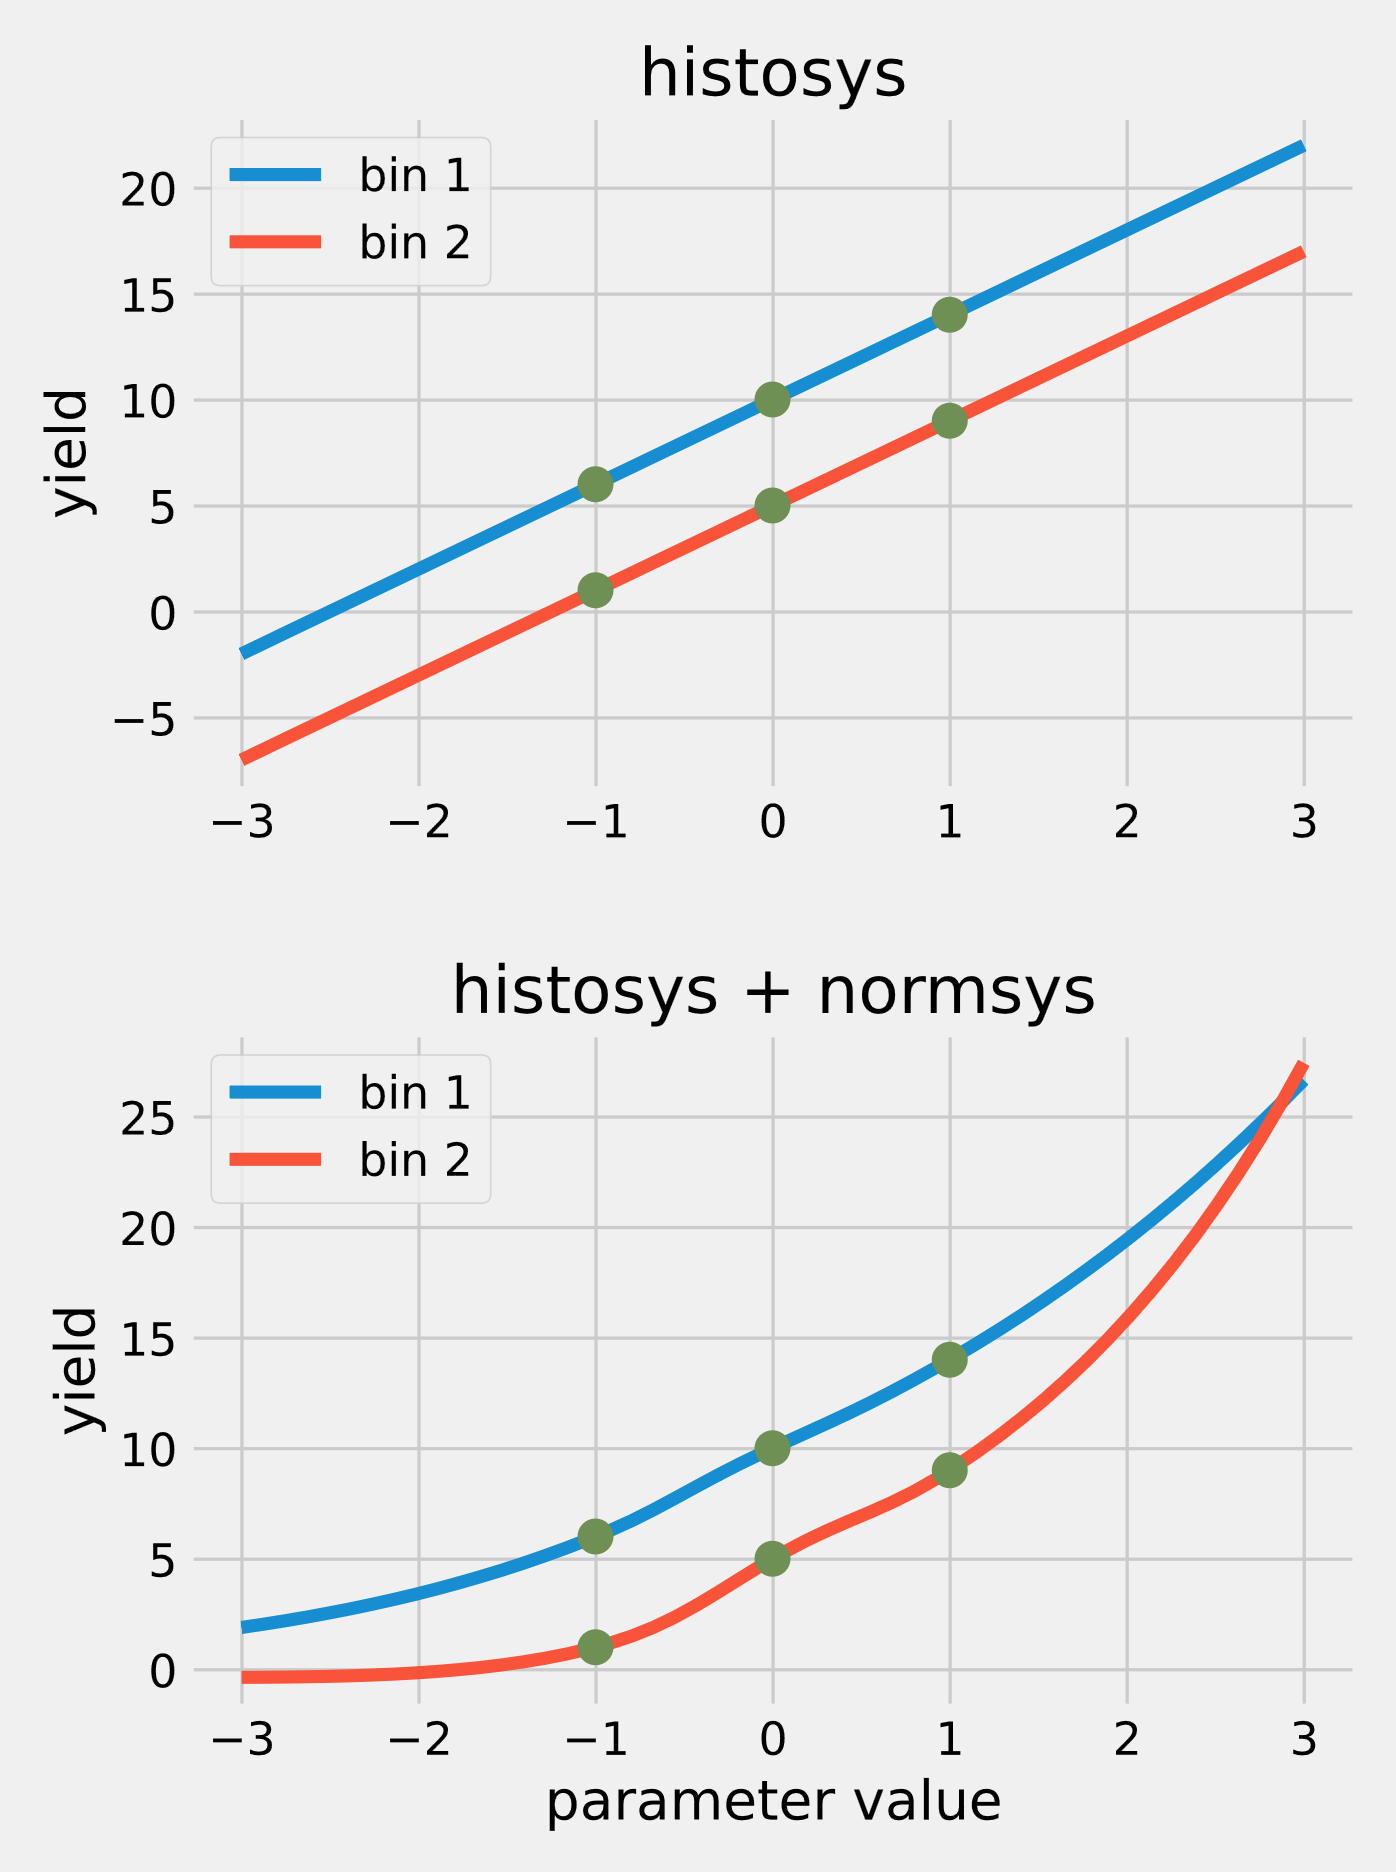
\includegraphics[width=.4\textwidth]{norm_shape}
    \caption[]{Effect of nuisance parameter pulling on histogram yields with and without applying an additional normalization uncertainty to a \textsc{HistoSys} shape uncertainty. Adopted from \citep{held_stat_intro}.}
    \label{fig:norm_shape}
\end{figure}


\section{Uncertainty Extraction}\label{sec:unc_extraction}
The standard error of a quantity is determined by measuring the square root of its variance. The covariance matrix is a generalization of variance for two random variables $X_i, X_j$
\begin{equation}
    V_{ij}=\text{Cov}(X_i, X_j) = \text{E}[(X_i - \text{E}[X_i])(X_j - \text{E}[X_j])].
\end{equation}
In the context of maximum likelihood estimation, the covariance matrix of the nuisance parameters $\bm{\theta}$ can be approximated in the large sample limit by the inverse of the negative Hessian of the log-likelihood function $L$
\begin{equation}
    V_{ij} =\left[ -\frac{\partial^2 L(\bm{\theta})}{\partial \theta_i \partial \theta_j} \right]^{-1}.
\end{equation}
The covariance matrix holds the variances and thus the uncertainties of the nuisance parameters along its diagonal, and the covariances between components off-diagonal. When propagating uncertainties, these covariances contribute to the overall uncertainty. This can be illustrated by examining the variance of a function $f(\theta_1, \theta_2)$ that depends on two parameters with individual $\sigma_1,\sigma_2$ uncertainties
\begin{equation}
    \text{Var}(f(\theta_1, \theta_2)) = \left( \frac{\partial f}{\partial \theta_1} \right)^2 \sigma_1^2 + \left( \frac{\partial f}{\partial \theta_2} \right)^2 \sigma_2^2 + 2 \left( \frac{\partial f}{\partial \theta_1} \right) \left( \frac{\partial f}{\partial \theta_2} \right) \sigma_{12}.
\end{equation}
If the parameters $\theta_1$ and $\theta_2$ are correlated the cross-term \(2 \left( \frac{\partial f}{\partial \theta_1} \right) \left( \frac{\partial f}{\partial \theta_2} \right) \sigma_{12}\) contributes to the overall uncertainty. Consequently, large correlations between parameters, indicated by significant off-diagonal terms, are disadvantageous for constraining the model.



















% \section{HistFactory}\label{sec
% }
% A widely-used model for constructing likelihoods, as discussed in Section \ref{sec
% }, is known as HistFactory \citep{cranmer2012histfactory}. HistFactory simplifies the process of building a likelihood by breaking it down into several fundamental components, considering a different categorization of the model parameters ϕϕ:
% \newcommand{\freeset}{\bm{\eta}}
% \newcommand{\constrset}{\bm{\chi}}
% \newcommand{\singleconstr}{\chi}
% \newcommand{\channelcounts}{\bm{n}}
% \newcommand{\auxdata}{\bm{a}}
% \newcommand{\poiset}{\bm{\psi}}
% \newcommand{\nuisset}{\bm{\theta}}
% \newcommand{\fullset}{\bm{\phi}}
% \newcommand{\singlefull}{\phi}
% \begin{equation}
%     L(\bm{x}|\fullset) \quad=\quad
%     L(\bm{x}|\overbrace{\poiset}^{\llap{\text{parameters of interest}}},\underbrace{\nuisset}{\llap{\text{nuisance parameters}}}) \quad=\quad
%     L(\bm{x}|\overbrace{\freeset}^{\rlap{\text{free}}},\underbrace{\constrset}{\rlap{\text{constrained}}}),
% \end{equation}
% into free parameters \freeset\freeset and constrained parameters \constrset\constrset, which incorporate uncertainties into the likelihood. Additionally, there may be several histograms of an observable, measured in orthogonal kinematic regions, called channels cc. Bins have the index bb, and constraint terms are denoted c\singleconstrc\singleconstr​. The likelihood can thus be described as:
% \begin{equation}
%     L(\channelcounts, \auxdata ,|,\freeset,\constrset)
%     = \underbrace{{\prod_{c\in\mathrm{,channels}} \prod_{b \in \mathrm{,bins}c}
%                 \textrm{Pois} (
%                 ;\overbrace{n{cb}}^{\llap{\text{\strut observed}\quad;}}
%                 ,|, \overbrace{\nu_{cb}\left(\freeset,\constrset\right)}^{\llap{\quad\text{\strut predicted}}}
%                 ;)}}{\substack{\text{Simultaneous measurement}\%
%             \text{of multiple channels}}}
%     \underbrace{{\prod{\singleconstr \in \constrset} c_{\singleconstr}(a_{\singleconstr} |, \singleconstr)}}_{\substack{\text{constraint terms}\%
%             \text{for }\text{auxiliary measurements}}}.
%     \label{eq
%     }
% \end{equation}
% Here, nn are observed and aa are the auxiliary measurement histograms. The ncbncb​ enter the Poisson term per bin and channel, where the predicted counts per bin are governed by the free and constrained parameters νcb(\freeset,\constrset)νcb​(\freeset,\constrset). The functions c\singleconstr(a\singleconstr∣ \singleconstr)c\singleconstr​(a\singleconstr​∣\singleconstr) penalize the likelihood LL with uncertainties aχaχ​ to constrain the parameter \singleconstr\singleconstr, as discussed in detail in Section \ref{sec
% }.

% The prediction is a sum of nominal counts per bin νscb0νscb0​ over all samples ss (e.g., tt‾tt, multijet-background, etc.). These nominal bin counts are subject to uncertainties and thus have some degree of freedom. However, the effect of this modification to the likelihood must be considered through the constraint terms, which penalize the likelihood proportional to the modification. Modifiers are discussed in detail in Section \ref{sec
% }. They enter the likelihood through linear modeling of the nominal bin content νscb0νscb0​ with multiplicative κscbκscb​ and additive modifiers ΔscbΔscb​:
% \begin{align}
%     \nu_{cb}\left(\freeset,\constrset\right) & = \sum_{s\in\mathrm{,samples}} \nu_{scb}\left(\freeset,\constrset\right) \
%                                              & = \sum_{s\in\mathrm{,samples}}\underbrace{\left(\prod_{\kappa\in,\bm{\kappa}} \kappa_{scb}\left(\freeset,\constrset\right)\right)}{\text{multiplicative modifiers}},
%     \Bigg(\nu{scb}^0 + \underbrace{\sum_{\Delta\in\bm{\Delta}} \Delta_{scb}\left(\freeset,\constrset\right)}_{\text{additive modifiers}}\Bigg).
%     \label{eq
%     }
% \end{align}
% This approach's usefulness becomes clear when considering one uncertainty aχaχ​ on a nominal bin count estimate νscb0νscb0​. The main goal remains to maximize the overall likelihood LL. This can be achieved by maximizing the Poisson probability in equation \ref{eq
% } while keeping the constraint term for uncertainties large. It is illustrative to consider one nuisance parameter χχ as a multiplicative modifier κscb=χκscb​=χ on νscb0νscb0​. An optimum can be found by modifying the prediction to move closer to the observed value while maintaining the constraint term controlled by the same χχ at values where the penalization of the likelihood stays insignificant.

% \subsection{Modifiers}\label{sec
% }
% In HistFactory, there are four types {λ,μ,γ,α}{λ,μ,γ,α} of multiplicative rate modifiers:

% Free rate modifiers for the luminosity λλ and signal strength μμ that affect all bins equally:
% \begin{equation}
%     \nu_{scb}(\mu)=\mu \nu_{scb}^0.
% \end{equation}
% These are bin-independent normalization factors that preserve the histogram's shape.

% Bin-wise modifiers γbγb​ (uncorrelated shape):
% \begin{equation}
%     \nu_{scb}(\gamma_b)=\gamma_b \nu_{scb}^0.
% \end{equation}
% These are useful for including uncertainties of a per bin data-driven background estimate.

% Interpolation parameters αα (shape factors) that enter the modeling through an interpolation function ηη instead of being the factor itself. They exist in multiplicative versions:
% \begin{equation}
%     \nu_{scb}(\alpha)=\eta(\alpha) \nu_{scb}^0,
% \end{equation}
% and additive versions:
% \begin{equation}
%     \nu_{scb}(\alpha)=\nu_{scb}^0 + \eta(\alpha).
% \end{equation}
% This is useful to include systematic uncertainties. Typically, they are known for one standard deviation of a count in a bin η−1=νscb1downη−1​=νscb1down​ and η1=νscb1upη1​=νscb1up​ to the nominal value νscb0νscb0​. These are then used to construct interpolation functions that modify the nominal value controlled by the nuisance parameter and control the constraint term cαcα​, further explained in Section \ref{sec
% }, such that one parameter controls the modification and constraint at a time.

% In HistFactory, there are four such interpolation functions. For these functions, there is an identity operator:
% \begin{equation}
%     \eta_0=\eta (\alpha=0) =
%     \begin{cases}
%         1 , & \text{multiplicative modifier, } (\kappa) \
%         0 , & \text{additive modifier, } (\lambda).
%     \end{cases}
% \end{equation}
% One example of these interpolation functions, which scales the count in a bin linearly over the known deviations η−1=νscb1downη−1​=νscb1down​ and η1=νscb1upη1​=νscb1up​, is:
% \begin{equation}
%     \eta_\mathrm{linear}(\alpha)=
%     \begin{cases}
%         \alpha(\eta_0 - \eta_1) ,    & \alpha>0 \
%         \alpha(\eta_0 - \eta_{-1}) , & \alpha<0
%     \end{cases}
% \end{equation}
% This is illustrated in Figure \ref{fig
% }(a). For other interpolation functions, see \citep{cranmer2012histfactory}. It is noted that αα is the nuisance parameter, not the function η(α)η(α), and there is an associated constraint term cαcα​ for each αα.

% \begin{figure}
%     \centering
%     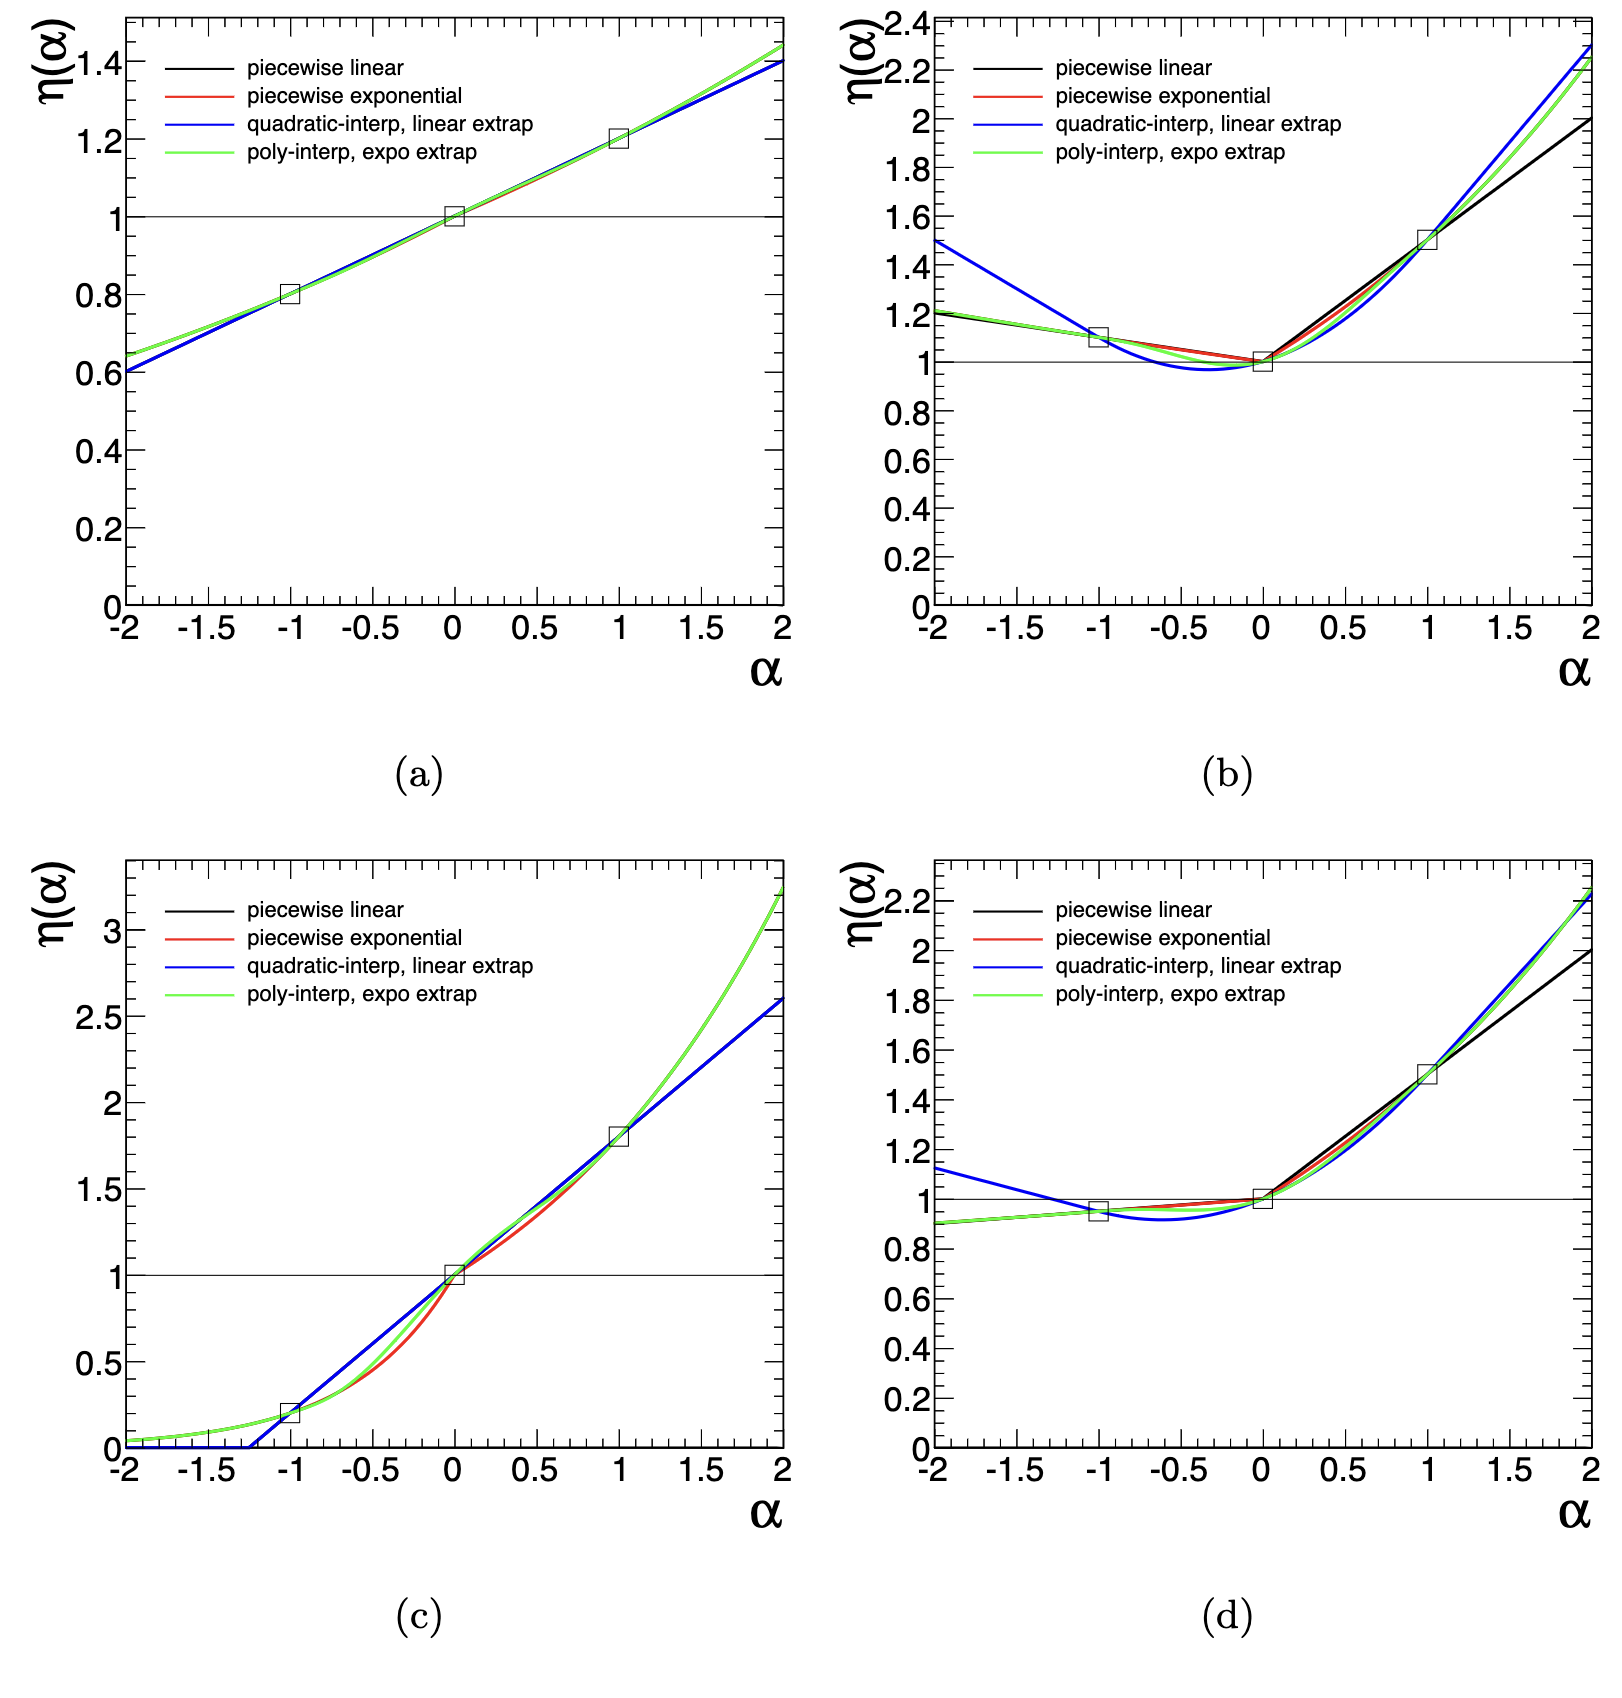
\includegraphics[width=.8\textwidth]{interp_func.png}
%     \caption[]{The four interpolation functions \eta(\alpha) for different up and down standard deviation values. For example, in (a), the bin count will be scaled by a factor of 0.8 for  (1.2 for α=1α=1). From \citep{cranmer2012histfactory}.}
%     \label{fig
%     }
% \end{figure}

% \subsection{Constraint Terms}\label{sec
% }
% Uncertainties are modeled either Gaussian or Poissonian. The Gaussian uncertainty implementation is straightforward as the standard deviation σσ appears in the definition of the Gaussian with mean μμ:
% \begin{equation}
%     \text{Gaus}(\mu|x,\sigma)=\frac{1}{\sigma\sqrt{2\pi}}e^{-\frac{1}{2}\left(\frac{x-\mu}{\sigma}\right)^2}.
% \end{equation}
% Thus, the likelihood for a Gaussian uncertainty is constrained by a Gaussian scaled to one standard deviation, controlled by the nuisance parameter αα: Gauss(α∣a,σ=1)Gauss(α∣a,σ=1).

% The Poisson distribution is given by:
% \begin{equation}
%     \text{Pois}(k|r)= \frac{r^k e^{-r}}{k!}.
% \end{equation}
% For a Poissonian-distributed uncertainty, the nuisance parameter for a multiplicative factor κscb=γκscb​=γ in equation \ref{eq
% } should control the Poisson constraint term such that the uncertainty σσ is reflected by the variance of the Poisson Var(Pois)=r=σ2Var(Pois)=r=σ2. This is achieved by scaling the distribution with a factor ff, which is then solved for the one with the desired uncertainty by evaluating it at the nominal value of the multiplicative modifier γ0=1γ0​=1:
% \begin{equation}
%     \mathrm{Var}\left[\mathrm{Pois}(k=f\gamma_0 | r=f\gamma)\right]
%     =
%     r=f\gamma;\stackrel{\gamma=\gamma_0}{=};f\gamma_0=(f\sigma)^2
%     \quad
%     \rightarrow \quad f=(1/\sigma^2).
% \end{equation}
% Thus, a Poissonian constraint term for a multiplicative modifier γγ with uncertainty σσ is Pois(k=σ−2∣r=σ−2γ)Pois(k=σ−2∣r=σ−2γ). This completes the necessities for the HistFactory model. The different types of modifiers and their constraint terms are summarized in Table \ref{tab
% }.

% \begin{table}[]
%     \caption[]{Modifiers and constraint terms used by HistFactory. Note that the interpolation functions are called fpfp​ and gpgp​ here instead of ηη as chosen in the full text. Input for the constraint terms are the corresponding uncertainties. Adapted from \citep{pyhf}.}
%     \centering
%     \resizebox{0.97\textwidth}{!}{
%         \begin{tabular}{l|l|l|l}\label{tab
%             }
%             Description          & Modification                                                          & Constraint Term c\singleconstrc\singleconstr​ & cχcχ​ input \
%             \hline
%             Uncorrelated Shape   & κscb(γb)=γbκscb​(γb​)=γb​                                             & ∏bPois(kb=σb−2| rb=σb−2γb)∏b​Pois(kb​=σb−2​

%             ​rb​=σb−2​γb​)       & σbσb​ \
%             Correlated Shape     & Δscb(α)=fp(α| Δscb,α=−1,Δscb,α=1)Δscb​(α)=fp​(α∣Δscb,α=−1​,Δscb,α=1​) & Gaus(a=0| α,σ=1)Gaus(a=0∣α,σ=1)               & Δscb,α=±1Δscb,α=±1​ \
%             Normalisation Unc.   & κscb(α)=gp(α| κscb,α=−1,κscb,α=1)κscb​(α)=gp​(α∣κscb,α=−1​,κscb,α=1​) & Gaus(a=0| α,σ=1)Gaus(a=0∣α,σ=1)               & κscb,α=±1κscb,α=±1​ \
%             MC Stat. Uncertainty & κscb(γb)=γbκscb​(γb​)=γb​                                             & ∏bGaus(aγb=1| γb,δb)∏b​Gaus(aγb​​=1∣γb​,δb​)  & δb2=∑sδsb2δb2​=∑s​δsb2​ \
%             Luminosity           & κscb(λ)=λκscb​(λ)=λ                                                   & Gaus(l=λ0| λ,σλ)Gaus(l=λ0​∣λ,σλ​)             & λ0,σλλ0​,σλ​ \
%             Normalisation        & κscb(μb)=μbκscb​(μb​)=μb​                                             &                                               & \
%             Data-driven Shape    & κscb(γb)=γbκscb​(γb​)=γb​                                             &                                               & \
%         \end{tabular}
%     }
% \end{table}
